%%%%%%%%%%%%%%%%%%%%%%%%%%%%%%%%%%%%%%%%%
% University Assignment Title Page 
% LaTeX Template
% Version 1.0 (27/12/12)
%
% This template has been downloaded from:
% http://www.LaTeXTemplates.com
%
% Original author:
% WikiBooks (http://en.wikibooks.org/wiki/LaTeX/Title_Creation)
%
% License:
% CC BY-NC-SA 3.0 (http://creativecommons.org/licenses/by-nc-sa/3.0/)
% 
% Instructions for using this template:
% This title page is capable of being compiled as is. This is not useful for 
% including it in another document. To do this, you have two options: 
%
% 1) Copy/paste everything between \begin{document} and \end{document} 
% starting at \begin{titlepage} and paste this into another LaTeX file where you 
% want your title page.
% OR
% 2) Remove everything outside the \begin{titlepage} and \end{titlepage} and 
% move this file to the same directory as the LaTeX file you wish to add it to. 
% Then add \input{./title_page_1.tex} to your LaTeX file where you want your
% title page.
%
%%%%%%%%%%%%%%%%%%%%%%%%%%%%%%%%%%%%%%%%%
%\title{Title page with logo}
%----------------------------------------------------------------------------------------
%	PACKAGES AND OTHER DOCUMENT CONFIGURATIONS
%----------------------------------------------------------------------------------------

\documentclass[12pt]{article}
\usepackage[margin=1in]{geometry}
\usepackage[english]{babel}
\usepackage[utf8x]{inputenc}
\usepackage{amsmath}
\usepackage{graphicx}
\usepackage[colorinlistoftodos]{todonotes}
\usepackage{natbib}


\usepackage{hyperref}
\begin{document}

\begin{titlepage}

\newcommand{\HRule}{\rule{\linewidth}{0.5mm}} % Defines a new command for the horizontal lines, change thickness here

\center % Center everything on the page
 
%----------------------------------------------------------------------------------------
%	HEADING SECTIONS
%----------------------------------------------------------------------------------------

\textsc{\LARGE Ukrainian Catholic University}\\[1cm] % Name of your university/college
\textsc{\Large Applied Sciences Faculty}\\[0.5cm] % Major heading such as course name
\textsc{\large Data Science Master Programme}\\[0.5cm] % Minor heading such as course title

%----------------------------------------------------------------------------------------
%	TITLE SECTION
%----------------------------------------------------------------------------------------

\HRule \\[0.4cm]
{ \huge \bfseries Kernel Principal Component Analysis and its Applications}\\[10pt]
{\Large \bfseries Project report}\\[0.4cm] % Title of your document
\HRule \\[1cm]
 
%----------------------------------------------------------------------------------------
%	AUTHOR SECTION
%----------------------------------------------------------------------------------------


% If you don't want a supervisor, uncomment the two lines below and remove the section above
\Large \emph{Authors:}\\
Irynei \textsc{Baran}\\Hanna \textsc{Pylieva}\\[1cm] % Your name

%----------------------------------------------------------------------------------------
%	DATE SECTION
%----------------------------------------------------------------------------------------

{\large \today}\\[2cm] % Date, change the \today to a set date if you want to be precise

%----------------------------------------------------------------------------------------
%	LOGO SECTION
%----------------------------------------------------------------------------------------


\includegraphics[height=4cm]{img/UCU-Apps.png}\\[1cm] % Include a department/university logo - this will require the graphicx package
 
%----------------------------------------------------------------------------------------

\vfill % Fill the rest of the page with whitespace

\end{titlepage}


\begin{abstract}
\todo{revise Abstract after finishing}
Principal component analysis (PCA) is a
popular tool for linear dimensionality reduction
and feature extraction. Kernel PCA
is the nonlinear form of PCA, which better
exploits the complicated spatial structure of
high-dimensional features. In this project, we
first review the basic ideas of PCA and kernel
PCA. Then we show some experimental
results to compare the performance
of kernel PCA and standard PCA for classification
problems. We also provide an overview of PCA and kPCA applications.
\end{abstract}

\section{Introduction}
\todo{rewrite the introduction}
In this section, we briefly review the principal component
analysis method, it's applications and limitations.

\section{Principal Component Analysis}
Principal component analysis, or PCA, is a mathematical procedure which is widely used for dimensionality reduction and feature selection. Those applications are achieved by projecting the data orthogonally onto a space with lower dimension, known as the principal subspace or feature space, such that the variance of projected data is maximal \citep*{bishop}.

Consider a data set $X$ containing $N$ observations of $D$ features ($D<N$). In order to visualize data or diminish number of features for modeling we want to reduce dimensionality of feature space to $M<D$. Whereas we are interested in most influential features to minimize data losses, that is why our goal is to maximize variance of projected data. The directions on which the data is projected called principal components. They are orthogonal and form coordinate system of subspace $M$ (see on ~\autoref{fig:pr-components}).

\begin{figure}
	\centering
	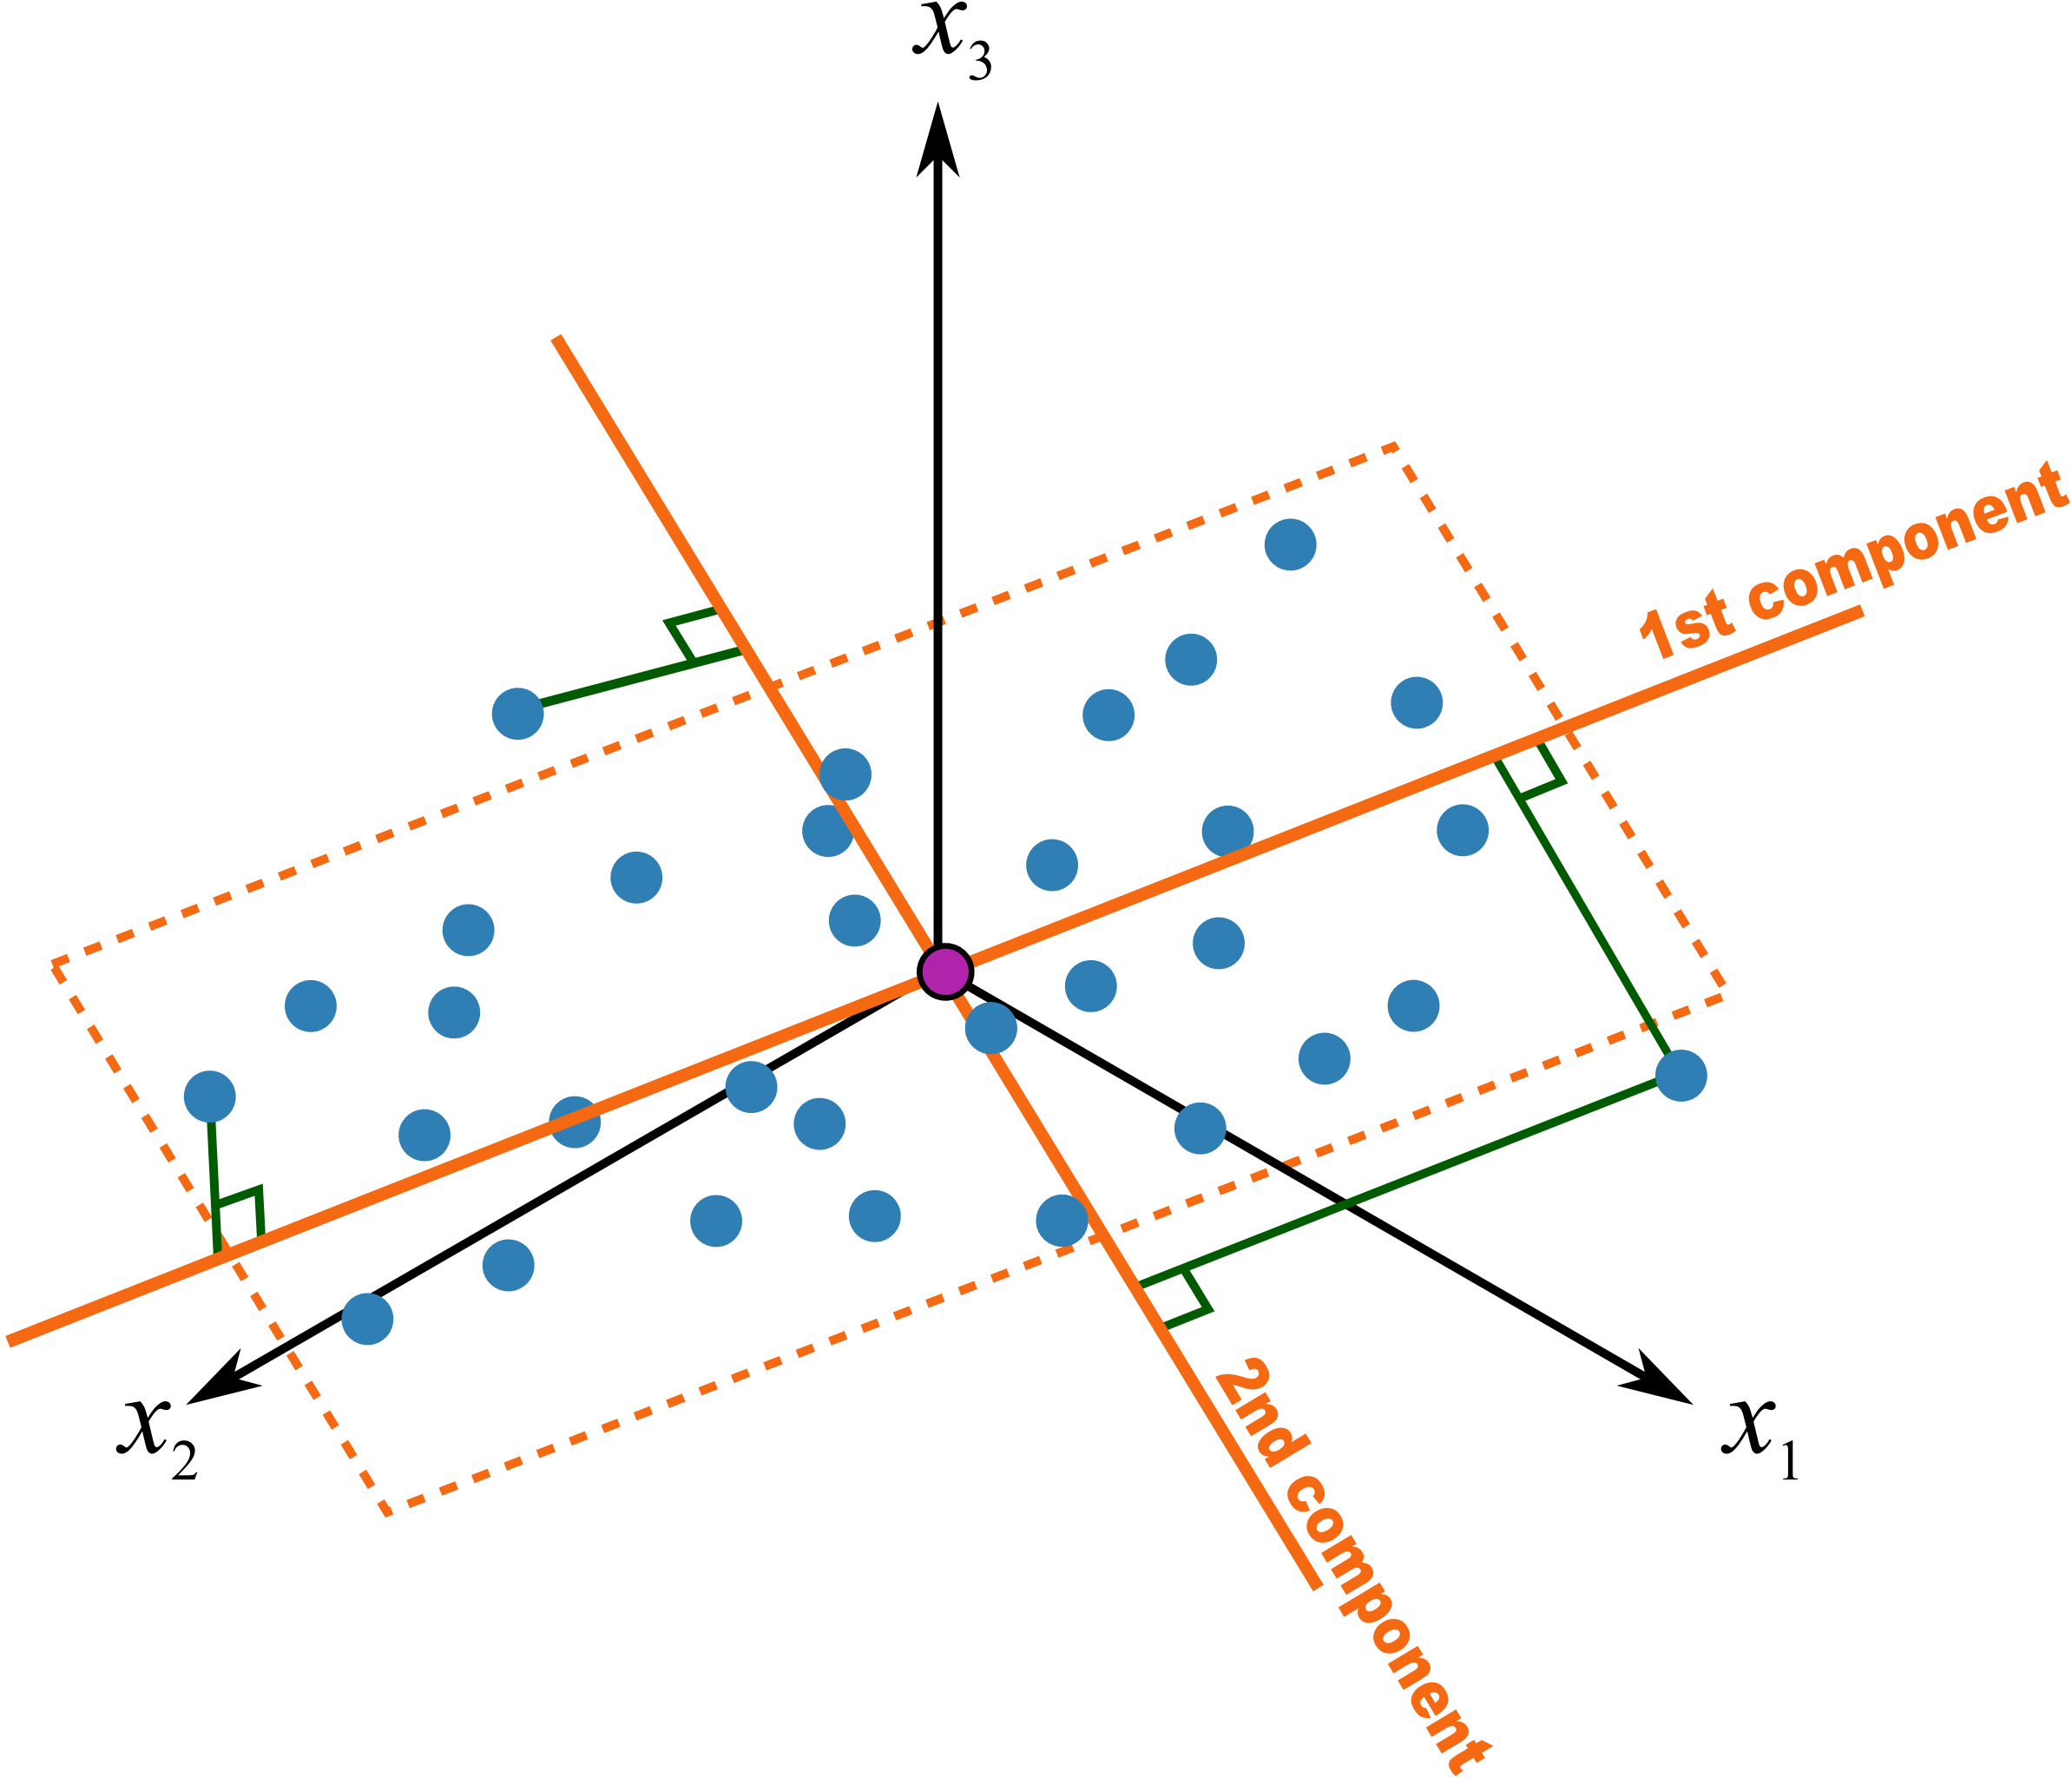
\includegraphics[scale=0.3]{img/geometric-PCA-8-both-components-with-plane.png}
	\caption{\label{fig:pr-components}Principal components}
\end{figure}

\subsection{Finding principal components}
To begin with, consider the projection on $M$ when $dim(M)=1$. Let a unit vector $u_1 \in D$ be the direction of $M$. Then projection of an observation $x_n\in X$ onto $M$ is $u_1^Tx_n$ and the variance of projected data is
\begin{equation}\label{var_proj}
 \dfrac{1}{N}\sum_{n=1}^{N}{\{u_1^T x_n - u_1^T \bar{x}\}}=u_1^T S u_1
\end{equation}	 
\todo[inline]{do we need to provide formula of covariance matrix explicitly? I don't feel so..}
where $\bar{x} = \frac{1}{N}\sum_{n=1}^{N} x_i$ is the mean of sample set and $S$ is the covariance matrix of data set $X$.

Maximization of \eqref{var_proj} is kept in a unit circle as we chose $u_1$ s.t. $||u_1||=u_1^T u_1=1$. So we need to find maximum of the next Lagrange function:
\begin{equation}
L(X,\lambda_1) = u_1^T S u_1 + \lambda_1(1-u_1^T u_1)
\end{equation}

By setting the derivative with respect to $u_1$ equal to zero we find that in stationary point $u_1$ needs to be an eigenvector of S:
\begin{equation}
S u_1 = \lambda_1 u_1
\end{equation}
Now when we left-multiply by $u^T_1$ and make use of $u^T_1 u_1 = 1$ we find out that the variance is given by
\begin{equation}
u_1^T S u_1 = \lambda_1 
\end{equation}
and so the variance will be a maximum when we set $u_1$ equal to the eigenvector
having the largest eigenvalue $\lambda_1$. This eigenvector id called the first principal
component \citep*{bishop}.

Next principal components can be found following the same procedure and choosing each new direction such that it maximizes the projected variance amongst all possible directions orthogonal to those already considered.

\todo[inline]{Do we need better explain the further procedure of it's clear enough?}

\subsection{Limitations of standard PCA}
Although PCA is very useful from practical prospective it has some limitations.
\begin{enumerate}
	\item Assumptions of linear dependency.
	PCA projects data orthogonally to reduce dimensionality. This works only if data has linear dependent variables:  $y = k x + \epsilon$. Otherwise the method doesn't identify the direction where  projected data has highest possible variance which can be seen on   ~\autoref{fig:pca-cons-demo-1} . 
	
	\begin{figure}
		\centering
		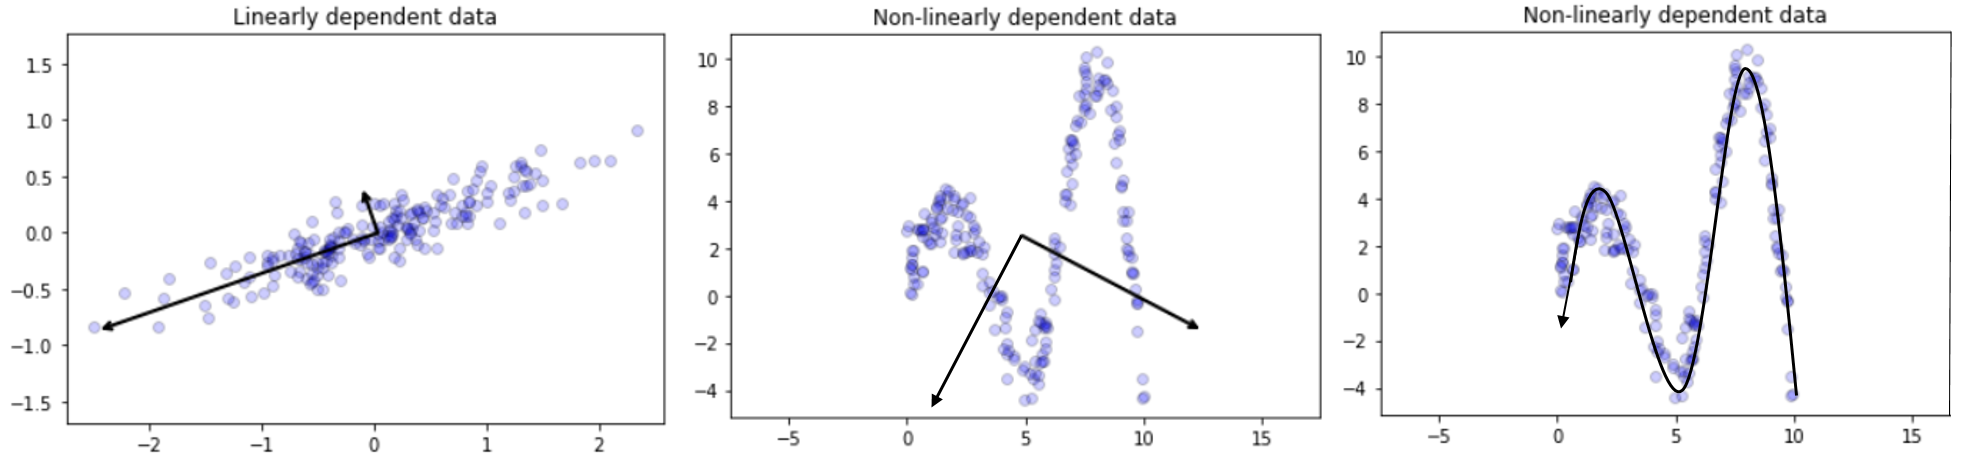
\includegraphics[scale=0.5]{img/pca-linear-separation-demo.png}
		\caption{\label{fig:pca-cons-demo-1}Demonstration of PCA's low performance for non-linearly dependent data}
	\end{figure}
	
	\item Spread maximization. 
	PCA searches for a subspace where projected data has the maximal spread. However, this is not always the best way to represent data in lower-dimension subspace. A common example is the task of separating and counting pancakes from an image (see ~\autoref{fig:pca-cons-demo-2}). Important information for the task (number of pancakes) is located along Z axis which has the lowest variance. So Z axis will be the last principal component identified by PCA which is not what required. 
	
	\begin{figure}
		\centering
		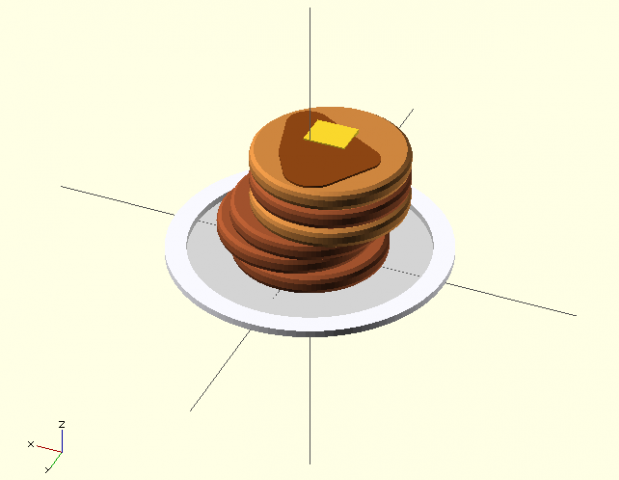
\includegraphics[width=.5\textwidth, scale=0.4]{img/pancakes.png}
		\caption{\label{fig:pca-cons-demo-2}Image from  \href{http://golancourses.net/2014/kevan/01/23/3d-parametric-pancakes/}{3D Parametric Pancakes}
		}
	\end{figure}
	
	\item Principal components are hard to interpret.
	PCA reveals implicit dependencies in data which is non-trivial to interpret in case of high-dimensional space reduction. The leverage for this issue is deep understanding of domain.
	
	\item Requirement of orthogonality.
	PCA comes up with orthogonal principal components, which do not overlap in the space. For some tasks such functionality will produce wrong results (see ~\autoref{fig:pca-cons-demo-3}).
	
	\begin{figure}
		\centering
		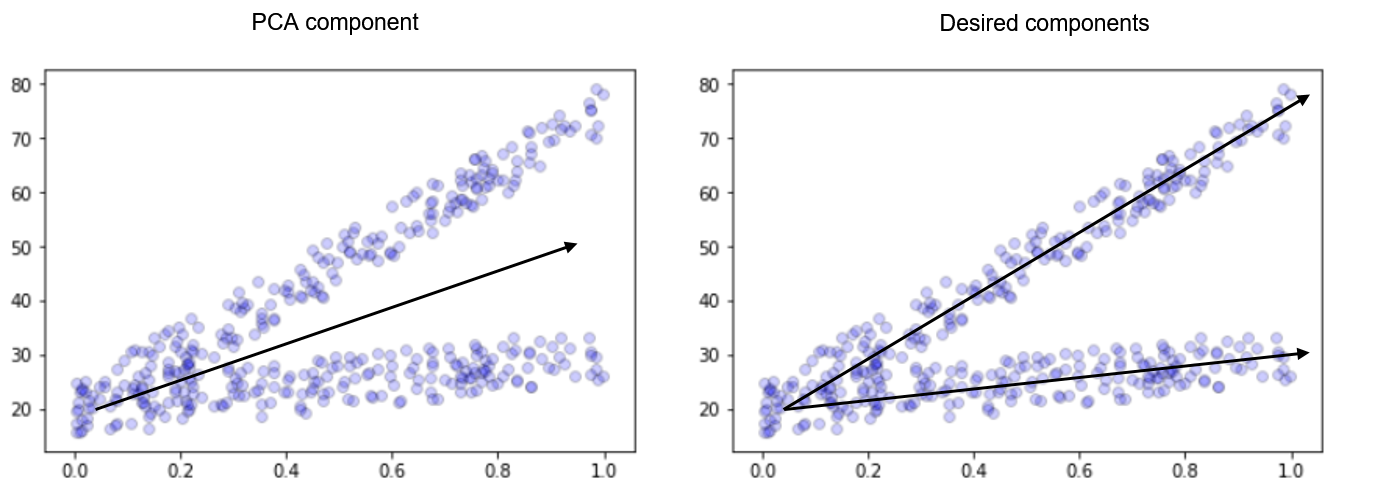
\includegraphics[scale=0.5]{img/non-orthogonal-components.png}
		\caption{\label{fig:pca-cons-demo-3}Demonstration of PCA's low performance for non-linearly dependent data}
	\end{figure}
	
\end{enumerate}

\subsection{Modifications of PCA}

\begin{thebibliography}{9}

\bibitem[Bishop (2006)]{bishop}
	Bishop, Christopher M.
	\textit{Pattern Recognition
	and Machine Learning.} Springer, Cambridge, U.K., 2006.
	
\end{thebibliography}

\end{document}